\documentclass[12pt]{article}
% This first part of the file is called the PREAMBLE. It includes
% customizations and command definitions. The preamble is everything
% between \documentclass and \begin{document}.

\usepackage[margin=1in]{geometry}  % set the margins to 1in on all sides
\usepackage{graphicx}              % to include figures
\usepackage{amsmath}               % great math stuff
\usepackage{amsfonts}              % for blackboard bold, etc
\usepackage{amsthm}                % better theorem environments

\usepackage{rotating} % for sideway table
\usepackage{xcolor}
\usepackage{hyperref}
\hypersetup{
    colorlinks,
    linkcolor={red!50!black},
    citecolor={blue!50!black},
    urlcolor={blue!80!black}
}
\usepackage{cleveref}

\usepackage{array,tabularx}
\usepackage{rotating}

\newenvironment{conditions*}
  {\par\vspace{\abovedisplayskip}\noindent
   \tabularx{\columnwidth}{>{$}l<{$} @{${}={}$} >{\raggedright\arraybackslash}X}}
  {\endtabularx\par\vspace{\belowdisplayskip}}
  
%\usepackage{float}
%\restylefloat{table} % Caption on top

% various theorems, numbered by section

\newtheorem{thm}{Theorem}[section]
\newtheorem{lem}[thm]{Lemma}
\newtheorem{prop}[thm]{Proposition}
\newtheorem{cor}[thm]{Corollary}
\newtheorem{conj}[thm]{Conjecture}

\DeclareMathOperator{\id}{id}

\newcommand{\bd}[1]{\mathbf{#1}}  % for bolding symbols
\newcommand{\RR}{\mathbb{R}}      % for Real numbers
\newcommand{\ZZ}{\mathbb{Z}}      % for Integers
\newcommand{\col}[1]{\left[\begin{matrix} #1 \end{matrix} \right]}
\newcommand{\comb}[2]{\binom{#1^2 + #2^2}{#1+#2}}

% bibliography
\usepackage{natbib}
\bibpunct{(}{)}{;}{a}{}{,} % no comma between author and year

\title{Prospectus updates}
\author{Anh Le}

\begin{document}
\maketitle

\section{Correlation between measures of corruption}

% latex table generated in R 3.2.1 by xtable 1.7-4 package
% Wed Jun 24 15:44:26 2015
\begin{table}[ht]
\centering
\begin{tabular}{rll}
  \hline
 & bureaucratic\_rents\_agree\_DDI & bribe\_size\_DDI \\ 
  \hline
bureaucratic\_rents\_agree\_DDI &  &  \\ 
  bribe\_size\_DDI &  0.51*** &  \\ 
  govcontract\_corrupt\_DDI & -0.10  & -0.16*  \\ 
   \hline
\end{tabular}
\caption{Correlation of year-on-year change across corruption measures, DDI} 
\label{tab:cor_corrupt_ddi}
\end{table}


% latex table generated in R 3.2.1 by xtable 1.7-4 package
% Wed Jun 24 15:44:26 2015
\begin{table}[ht]
\centering
\begin{tabular}{rlll}
  \hline
 & bureaucratic\_rents\_agree\_FDI & bribe\_size\_FDI & custom\_corrupt\_FDI \\ 
  \hline
bureaucratic\_rents\_agree\_FDI &  &  &  \\ 
  bribe\_size\_FDI &  0.33  &  &  \\ 
  custom\_corrupt\_FDI &  0.19  &  0.53**  &  \\ 
  govcontract\_corrupt\_FDI & -0.28  &  0.77*  &  0.72*  \\ 
   \hline
\end{tabular}
\caption{Correlation of year-on-year change across corruption measures, FDI} 
\label{tab:cor_corrupt_fdi}
\end{table}


\section{Regression: The relationship between corruption and spill-over effect}

\begin{itemize}
\item Bureaucratic corruption: Fraction of firms agreeing that provinces use inspections to extract fees, FDI, province-year
\item Custom corruption: Fraction of firms reporting paying bribe at port, FDI, province-year
\item Bribe size: Average informal fees as \% of firms' revenue, FDI, province-year
\item Registration corruption: Fraction of firms engaging in registration corruption, FDI, province. Firms in restricted industries, i.e. those approved by the PM office instead of by provinces, are excluded.
\item Procurement corruption: Fraction of firms reporting paying bribe at port, FDI, province-year
\end{itemize}


% Table created by stargazer v.5.1 by Marek Hlavac, Harvard University. E-mail: hlavac at fas.harvard.edu
% Date and time: Wed, Jun 24, 2015 - 04:09:41 PM
% Requires LaTeX packages: rotating 
\begin{sidewaystable}[!htbp] \centering 
  \caption{Relationship between FDI corruption and spill-over effect. Hierarchical model with varying intercepts for provinces and survey years} 
  \label{tab:pci_corruption} 
\small 
\begin{tabular}{@{\extracolsep{5pt}}lccccc} 
\\[-1.8ex]\hline 
\hline \\[-1.8ex] 
 & \multicolumn{5}{c}{\textit{Dependent variable:}} \\ 
\cline{2-6} 
\\[-1.8ex] & \multicolumn{5}{c}{\% of sale to foreign firms} \\ 
\\[-1.8ex] & \multicolumn{5}{c}{\textit{linear}} \\ 
 & \multicolumn{5}{c}{\textit{mixed-effects}} \\ 
\\[-1.8ex] & (1) & (2) & (3) & (4) & (5)\\ 
\hline \\[-1.8ex] 
 equity size & $-$0.149 & $-$0.152 & $-$0.145 & $-$0.150 & $-$0.706$^{**}$ \\ 
  & (0.230) & (0.230) & (0.230) & (0.226) & (0.359) \\ 
  labor size & 0.889$^{***}$ & 0.912$^{***}$ & 0.888$^{***}$ & 0.866$^{***}$ & 1.090$^{***}$ \\ 
  & (0.253) & (0.253) & (0.253) & (0.248) & (0.416) \\ 
  bureaucratic corruption & 8.557$^{***}$ &  &  &  &  \\ 
  & (3.195) &  &  &  &  \\ 
  custom corruption &  & 9.074$^{***}$ &  &  &  \\ 
  &  & (2.985) &  &  &  \\ 
  bribe size &  &  & 1.879 &  &  \\ 
  &  &  & (1.227) &  &  \\ 
  registration corruption &  &  &  & $-$2.822 &  \\ 
  &  &  &  & (2.270) &  \\ 
  procurement corruption &  &  &  &  & 0.106 \\ 
  &  &  &  &  & (0.662) \\ 
  log(\# of domestic firms per 1000 people) & 0.987 & 0.363 & 0.986 & 0.853 & 2.504 \\ 
  & (1.111) & (1.098) & (1.149) & (1.114) & (2.044) \\ 
  log population & 1.328 & 0.450 & 1.385 & 1.308 & 3.733 \\ 
  & (1.434) & (1.450) & (1.466) & (1.426) & (2.786) \\ 
  log GDP & $-$0.646 & $-$1.064$^{**}$ & $-$0.925$^{*}$ & $-$0.829$^{*}$ & $-$0.909 \\ 
  & (0.493) & (0.483) & (0.489) & (0.486) & (0.850) \\ 
  log distance to HN / HCMC & 0.167 & $-$0.090 & 0.098 & 0.184 & 0.671 \\ 
  & (0.427) & (0.422) & (0.441) & (0.443) & (0.754) \\ 
  Constant & $-$15.793 & $-$1.866 & $-$15.073 & $-$9.680 & $-$41.321 \\ 
  & (18.990) & (18.641) & (19.799) & (18.886) & (35.578) \\ 
 \hline \\[-1.8ex] 
Industry fixed effect (ISIC 2-digit) & Yes & Yes & Yes & Yes & Yes \\ 
Ownership type fixed effect & Yes & Yes & Yes & Yes & Yes \\ 
\hline \\[-1.8ex] 
Observations & 5,969 & 5,969 & 5,969 & 6,086 & 2,869 \\ 
Log Likelihood & $-$25,380.330 & $-$25,379.640 & $-$25,383.650 & $-$25,832.870 & $-$12,353.010 \\ 
\hline 
\hline \\[-1.8ex] 
\textit{Note:}  & \multicolumn{5}{r}{$^{*}$p$<$0.1; $^{**}$p$<$0.05; $^{***}$p$<$0.01} \\ 
\end{tabular} 
\end{sidewaystable} 


\section{Visualize regressions}

These two graphs visualize the positive effect of \textit{bureaucratic corruption} and \textit{custom corruption} above.

The x-axis represents the level of corruption. The y-axis represents the residuals of the \% sale to FDI firms in models with full controls but no corruption. It represents the part of spillover effect that is unexplained by the controls.

\begin{figure}[!ht]
\centering
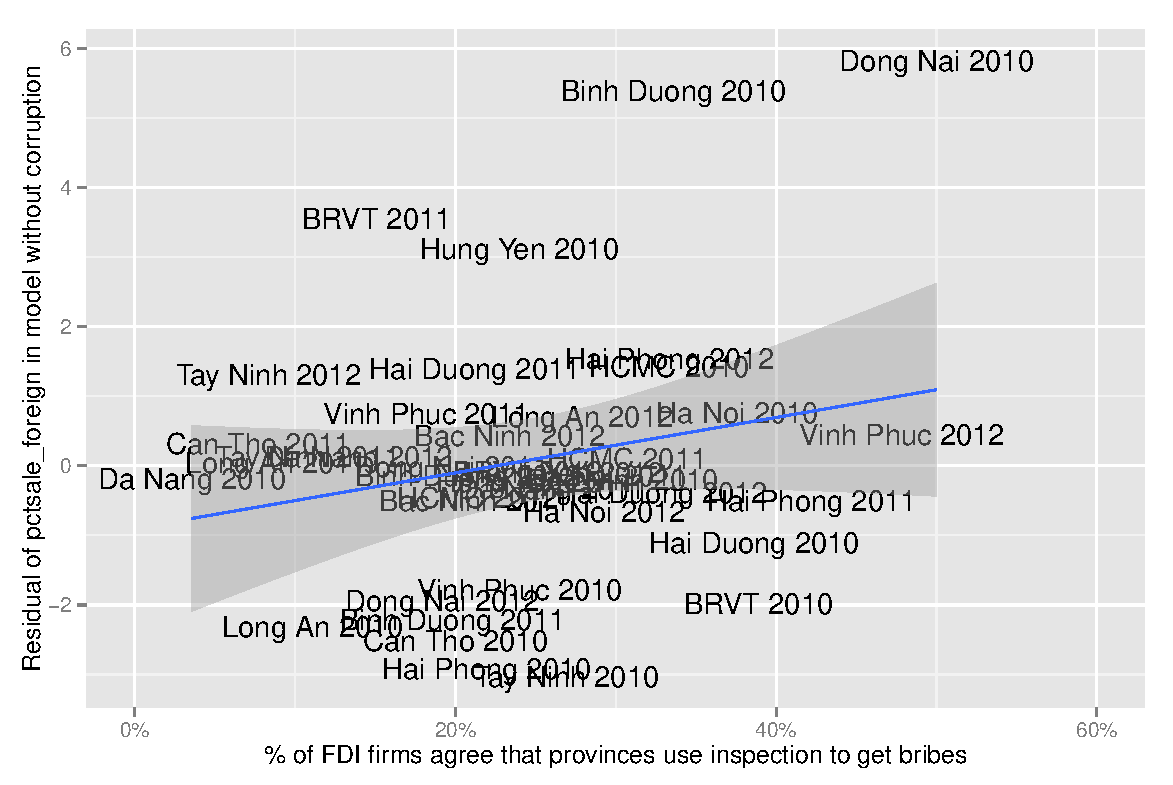
\includegraphics[width=\textwidth, height=\textheight,keepaspectratio]{../figure/bureaucratic_rents_residual}
\caption{Effect of bureaucratic corruption on spillover}
\end{figure}

\begin{figure}[!ht]
\centering
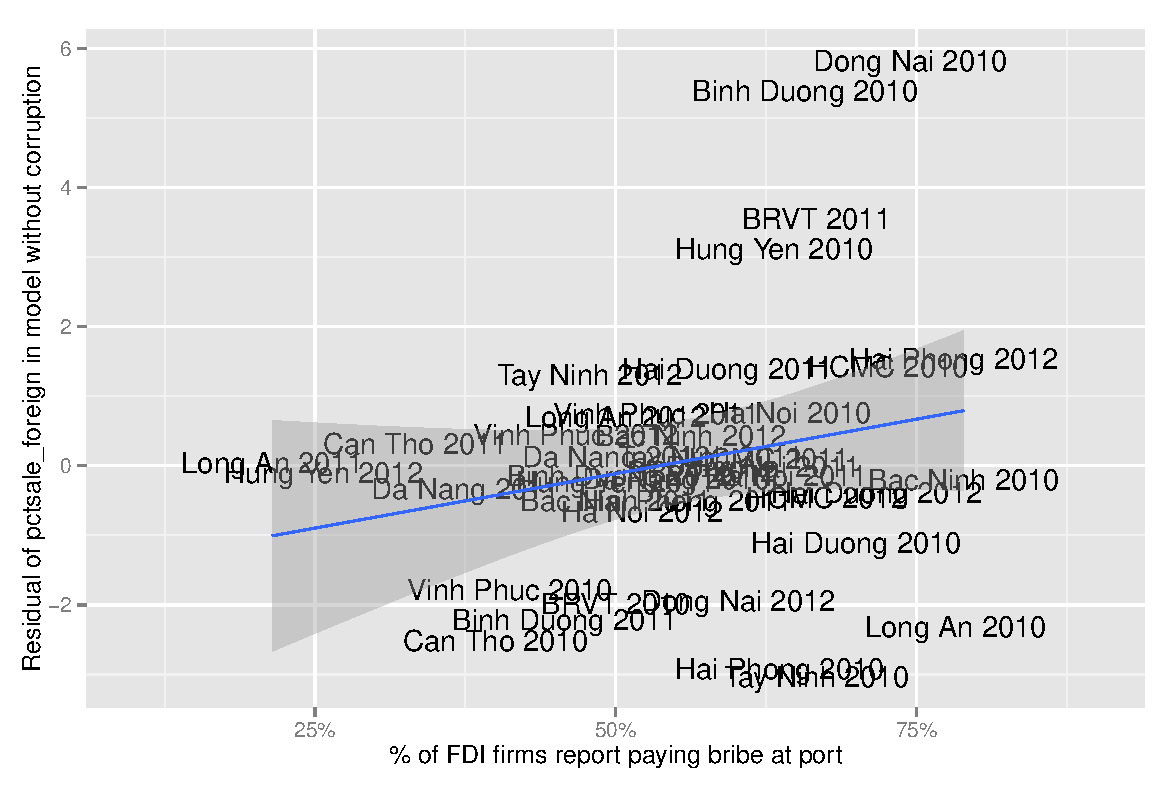
\includegraphics[width=\textwidth, height=\textheight,keepaspectratio]{../figure/custom_corrupt_residual}
\caption{Effect of custom's corruption on spillover}
\end{figure}


\end{document}